\documentclass[12pt]{article}
\usepackage{hyperref}
\usepackage{authblk}
\usepackage{graphicx}
\usepackage{amsmath}
\usepackage{amssymb}
\usepackage{enumitem}
\usepackage{amsfonts}
\usepackage{array}
\usepackage{xcolor}
\usepackage{tikz}
\usepackage{pifont}
\usepackage{fontawesome5}
\usepackage{tikz-3dplot}
\usepackage{forest}
\usepackage{cancel}
\usepackage{ulem}
\usepackage{subcaption}
\usepackage{booktabs}
\usepackage{placeins}
\usepackage[margin=1in]{geometry}

\title{Methodology of Creating SVM Kernels from Scratch Using Python and NumPy}
\author{Austin Lackey}
\author{Tomy Sabalo Farias}
\affil{DSCI 320, Colorado State University}

\begin{document}

\maketitle

\begin{abstract}
This paper presents a methodology for creating Support Vector Machine (SVM) kernels from scratch using Python and NumPy. 
We discuss the implementation of linear, sigmoid, polynomial, and radial basis function (RBF) kernels in a binary and multiclass SVM.
These kernels are tested on E. coli data and compared to the results of the scikit-learn SVM implementation.
The goal of the E. coli dataset is to predict the localization sites of proteins inside the cell. 
The results show that the implemented kernels will sometimes yield better accuracy than the scikit-learn implementation; at the
cost of increased training time. Kernel training times are run multiple times and averaged to provide a more accurate
metric since training times are low and have a high variance.
\end{abstract}

\section{Introduction}

Support Vector Machines (\textbf{SVMs}) are machine learning algorithms that are used to complete classification tasks. When we have a large dimensional data set that we would like to create decision boundaries, we can create a hyperplane that maximizes the margin between the observations' labels. The data points that are closest to the decision boundary influence the position and direction of the hyperplane, and these close data points are called \textbf{Support Vectors}. The goal is to optimize the distance between the support vectors and the hyperplane (also known as the \textbf{margin}), so we can draw a line between the points.

With higher dimensional data, sometimes a linear boundary will not be effective, and so we can implement kernel tricks. These kernels allow for the original input to be mapped to a higher-dimensional space where a linear boundary can be drawn. We will demonstrate the usage of SVMs and the effect that different kernels have on the same data. 

\section{Methodology}

When discussing SVMs, we need to understand the steps behind the math to know what it is doing. Here, we will discuss how this algorithm calculates our optimal parameters for our hyperplane decision boundary.

Our goal is to find a hyperplane in the form:
$$f(x) = w \cdot x + b = 0$$

We want our decision boundary to have a maximal margin between the hyperplane and the support vectors. These vectors are found with:
$$w \cdot x + b \geq 1$$
$$w \cdot x + b  \leq -1$$
Since we want to maximize the margin in between, we can think about finding those inputs that satisfy the support vectors in the right labels. For example, if we find an $x_n$ such that it is the $n$th observation in the dataset, and it has the label $y_n = 1$, then we want this observation to be found above the positive support vector. Mathematically, we can say that:
$$\begin{cases}
      w \cdot x + b \geq 1 & \text{if } y = 1 \\
      w \cdot x + b \leq -1 & \text{if } y = -1
\end{cases}$$
In other words, we can simply this to be:

$$y_i (w \cdot x_i + b) \geq 1$$ for $i = 1,...,N$

The support vectors are described, but we want to find the maximum length a unit step takes from the decision boundary to the support vectors to be optimized. Therefore, if we are given a vector $x$, with an orthogonal vector $w$ to the decision boundary, we can take a unit step from the decision boundary to the support vector by:
$$1 = w \cdot x + b = w(x + \frac{w}{|w|^2}) + b = 1$$

We know that $w \cdot x + b = 0$, so we can simplify:
$$\frac{ww}{|w|^2} = 1$$
$$\frac{1}{|w|}$$
This represents half the margin of the SVM, and so we need to do it to both sides of the boundary:
$$\frac{2}{|w|}$$
Therefore, to maximize the margin of the hyperplane, we need to minimize $w$.

We can combine this all to formulate our optimization problem: minimize $||w||$ constrained by $y_i (w \cdot x_i + b) \geq 1$ for $i = 1,..., N$.
We can set up a Lagrange dual optimization problem, such that:
$$L = \frac{1}{2}||w||^2 - \sum_{i=1}^{n} \alpha_i \cdot [y_i(w \cdot x + b) - 1]$$
Minimizing for $w$ and $b$, we get:
$$w = \sum_{i=1}^{n} \alpha_i y_i x_i$$
$$\sum_{i=1}^{n} \alpha_i y_i = 0$$

Our problem can now be in terms of a constrained minimization problem by plugging in the constraints we have. This can be simplified into a quadratic form. The final form of our problem will be

\begin{equation}
    L = 1^T \alpha - \frac{1}{2}\alpha^TX^TX\alpha
\end{equation}

\subsection{Kernel Functions}
We implemented four different kernel functions which are listed below.
\begin{itemize}
    \item Linear Kernel
    \begin{equation}
    K(X, Y) = X^T Y
    \end{equation}
    
    \item Sigmoid Kernel
    \begin{equation}
    K(X, Y) = \tanh(\gamma X^T Y + r)
    \end{equation}
    
    \item Polynomial Kernel
    \begin{equation}
    K(X, Y) = (\gamma X^T Y + r)^d, \gamma > 0
    \end{equation}
    
    \item Radial Basis Function (RBF) Kernel
    \begin{equation}
    K(X, Y) = \exp(-\gamma ||X - Y||^2), \gamma > 0
    \end{equation}
\end{itemize}

The kernel tricks used to form a linear decision boundary on a non-linear data set will be implemented into the optimization problem (1). For the linear kernel, no difference is made because it is the same thing that is done in the equation, just the product of the inputs. However, for the other kernels, the trick is implemented in the transformation of the input:
$$(X^TX)_{ij} = \sum_{d} y_i x_{id} \cdot y_j x_{jd} = \sum_{d} y_i y_k \cdot x_{id} x_{jd}$$
$$(k^Tk)_{ij} = \sum_{d'} y_i k_{id'} \cdot y_j k_{jd'} = \sum_{d'} y_i y_k \cdot k_{id'} k_{jd'}$$

The $k$ is found using the different kernel equations [(2)-(5)], which allows for versatility in the shape of the boundary line. It is the optimal decision boundary that contains 

\subsection{Binary SVM}

A binary classification of the data is the foundation of the calculations. We want to form a hyperplane that separates two labels effectively, with a margin for error when making predictions on new observations. The steps to complete to find the terms for our hyperplane can be seen below:

\begin{itemize}
    \item For each training example $(\mathbf{x}_i, y_i)$:
    \begin{itemize}
        \item Calculate error $E_i$ for $\mathbf{x}_i$ using the current model:
        \begin{equation*}
            E_i = f(\mathbf{x}_i) - y_i
        \end{equation*}
        \begin{equation*}
            f(x_i) = \sum_{j=1}^n \alpha_i y_i K (x_j,x_i) + b
        \end{equation*}
        \item If $(y_i \cdot E_i < -tol \text{ and } \alpha_i < C)$ or $(y_i \cdot E_i > tol \text{ and } \alpha_i > 0)$:
        \begin{itemize}
            \item Select a second example $(\mathbf{x}_j, y_j)$ to update alpha (using heuristics to choose $j \neq i$)
            \item Calculate error $E_j$ for $\mathbf{x}_j$
            \item Save old alpha values: $\alpha_i^{old} = \alpha_i$, $\alpha_j^{old} = \alpha_j$
            \item Compute bounds $L$ and $H$ for $\alpha_j$ (satisfying $0 \leq \alpha_j \leq C$)
            \item If $L$ equals $H$, continue to the next training example
            \item Compute $\eta$ (second derivative of the SVM objective function)
            \item Update $\alpha_j$:
            \begin{align*}
                \alpha_j &= \alpha_j^{old} - \frac{y_j \cdot (E_i - E_j)}{\eta} \\
                &\text{(Clip $\alpha_j$ if necessary: $\alpha_j = \text{clip}(\alpha_j, L, H)$)} \\
                &\text{(Continue if $|\alpha_j - \alpha_j^{old}| < \text{epsilon}$)}
            \end{align*}
            \item Update $\alpha_i$:
            \begin{equation*}
                \alpha_i = \alpha_i^{old} + y_i \cdot y_j \cdot (\alpha_j^{old} - \alpha_j)
            \end{equation*}
            \item Update bias term $b$ (compute $b_1$ and $b_2$, adjust $b$ based on $\alpha_i$ and $\alpha_j$, update $E$ for all examples)
        \end{itemize}
    \end{itemize}
\end{itemize}

Using this algorithm, you can find the $w$'s and $b$ that define the hyperplane between the two classes. The $K()$ function represents the kernel that is being used, and so this is where the different transformations will have an effect. 

\subsection{Multiclass SVM}
The multi-classification on a data set using SVM is only a slight variation from the binary classification. In binary, we trained the model on a \textbf{1 vs 1} basis. We had two classes, -1 and 1, and wanted to create a decision boundary between them. However, multiple classes mean that we have more than two classes, and you can't just draw one line to separate the labels.

Therefore, the meta-algorithm for multi-class is to approach with a \textbf{one vs others} mindset. For however many classes you have, you want to create a decision boundary between one class and all the others and repeat this until you have done so for each label. It follows the same steps as binary classification, but does it $s$ times for the number of labels in the data set to differentiate. 
\section{Data Overview}
The data is composed of seven predictors of type float, with the last column being the localization site class label.
There were 336 total observations in the data set, and the class labels were not evenly distributed.
As you can see below, the class labels \textit{cp} and \textit{im} make up the majority of the data set.
We used these two classes as the positive and negative classes for the binary SVMs as they were the most common.
\begin{table}[h]
    \centering
    \caption{Class Frequency}
    \label{tab:class_frequency}
    \begin{tabular}{cc}
        \toprule
        \textbf{Class} & \textbf{Frequency} \\
        \midrule
        cp & 143 \\
        im & 77 \\
        pp & 52 \\
        imU & 35 \\
        om & 20 \\
        omL & 5 \\
        imS & 2 \\
        imL & 2 \\
        \bottomrule
    \end{tabular}
\end{table}
For a test/train split, we used 80\% of the data for training and 20\% for testing.
This resulted in 268 training observations for the multi-class SVMs and 176 training observations for the binary SVMs.
\section{Results and Discussion}
\subsection{Training Time and Accuracy}
After implimenting the SVM kernels for both binary and multiclass classification, we tested the kernels on the E. coli data set.
Since training times were low and had a higher variance, we ran each kernel 10 times and averaged the results.
This allows for a more accurate representation of the training time for each kernel to prevent outliers from skewing the results.
The results of the training times and accuracy can be seen in Table \ref{tab:classifier_performance}.
\begin{table}[h]
    \centering
    \caption{Classifier Performance}
    \label{tab:classifier_performance}
    \begin{tabular}{cccccc}
        \toprule
        \textbf{Classifier} & \textbf{Implementation} & \textbf{Kernel} & \textbf{Avg Accuracy} & \textbf{Avg Runtime} \\
        \midrule
        Binary & sklearn & linear & 1 & 0.00119 \\
        Binary & custom & linear & 0.99318 & 0.00719 \\
        Binary & sklearn & sigmoid & 0.6818 & 0.00069 \\
        Binary & custom & sigmoid & 0.95908 & 0.05421 \\
        Binary & sklearn & rbf & 1 & 0.00034 \\
        Binary & custom & rbf & 0.99546 & 0.00773 \\
        Binary & sklearn & poly & 1 & 0.00035 \\
        Binary & custom & poly & 0.95909 & 0.00926 \\
        Multi & sklearn & linear & 0.7794 & 0.00094 \\
        Multi & custom & linear & 0.81762 & 0.13374 \\
        Multi & sklearn & sigmoid & 0.4706 & 0.00199 \\
        Multi & custom & sigmoid & 0.68826 & 1.50449 \\
        Multi & sklearn & rbf & 0.8824 & 0.00111 \\
        Multi & custom & rbf & 0.82939 & 0.17472 \\
        Multi & sklearn & poly & 0.8529 & 0.00107 \\
        Multi & custom & poly & 0.84849 & 0.32641 \\
        \bottomrule
    \end{tabular}
    \vspace{1em}  % Add some vertical space for the note
    \begin{tabular}{p{0.9\textwidth}}  % Create a new table for the note
        \multicolumn{1}{l}{\textit{Note:}} These times were calculated with 10 runs for each kernel and averaged. \\
    \end{tabular}
\end{table}
\FloatBarrier 
I think that the results are interesting because the custom implementation of the kernels often outperformed the scikit-learn implementation.
However, the custom implementation of the kernels took significantly longer to train. Since we used Stochastic Gradient Descent (SGD) to train the SVMs, 
the convergence can take a long time. In Sklearn, they use LibSVM which is a C++ library that is much faster than our custom implementation.
Although the multi-class SVMs had lower accuracy than the binary SVMs, the training times were much higher. This makes sense because the multi-class SVMs
are just a combination of binary SVMs and the decision boundaries start to become more complex and harder to fit accurately.
\FloatBarrier 
\subsection{Decision Boundaries}
The decision boundaries for the binary and multi-class SVMs can be seen in Figures 1 and 2.
In Figure 1, the decision boundaries for the binary SVMs are shown. We can see how each kernel affects the decision boundary.
Although these examples are intuitive and easy to understand, the data was reduced to 2 dimensions using Principal Component Analysis (PCA).
We decided to use PCA to reduce the dimensionality of the data because we knew that the training data would retain more information than 
regular feature selection. By implementing feature extraction, we were able to reduce the dimensionality of the data while retaining more information.
This allows us to show the decision boundaries in 2 dimensions while still retaining the accuracy of the SVMs.

For the binary SVMs, we selected the classes \textit{cp} and \textit{im} to be the positive and negative classes respectively.
We can see that the linear kernel has a linear decision boundary which is expected and the rest of the kernels have non-linear decision boundaries.
\begin{figure}
    \centering
    \begin{subfigure}{0.45\textwidth}
        \centering
        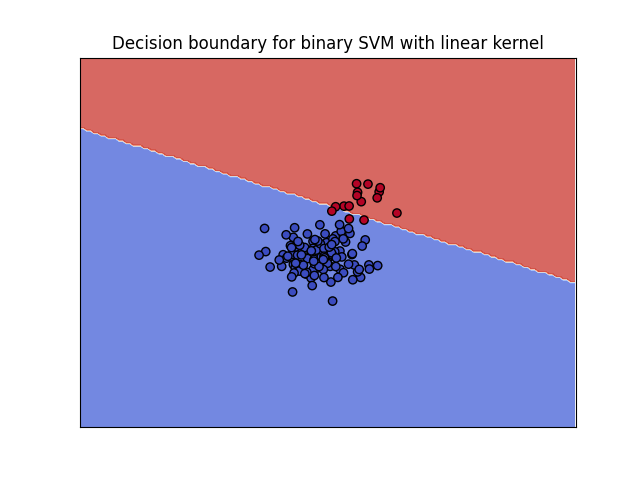
\includegraphics[width=\textwidth]{plots/linear_binary.png}
        \caption{Linear Binary SVM}
    \end{subfigure}
    \begin{subfigure}{0.45\textwidth}
        \centering
        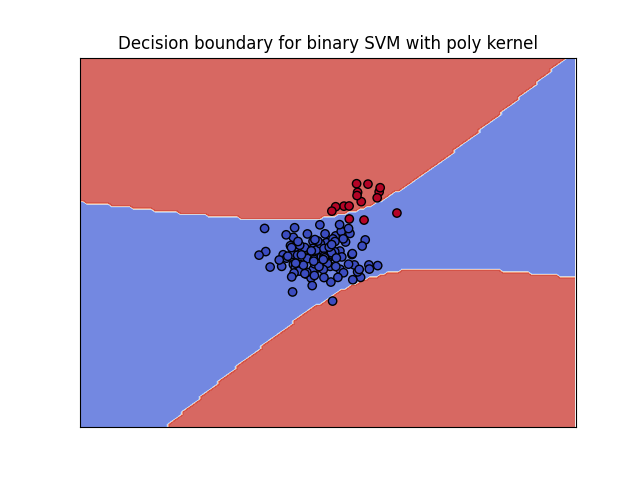
\includegraphics[width=\textwidth]{plots/poly_binary.png}
        \caption{Polynomial Binary SVM}
    \end{subfigure}
    \begin{subfigure}{0.45\textwidth}
        \centering
        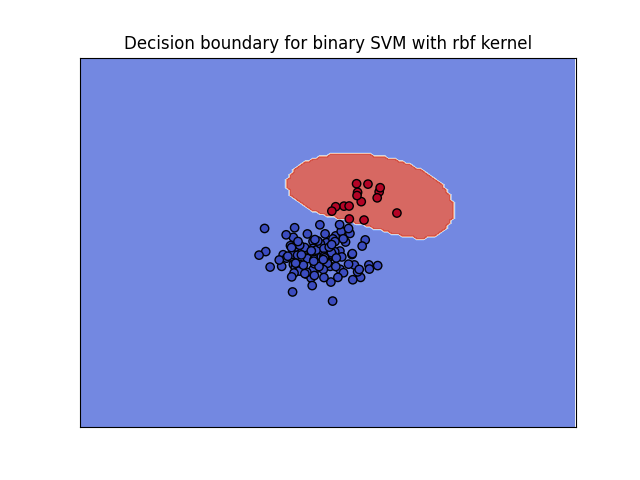
\includegraphics[width=\textwidth]{plots/rbf_binary.png}
        \caption{RBF Binary SVM}
    \end{subfigure}
    \begin{subfigure}{0.45\textwidth}
        \centering
        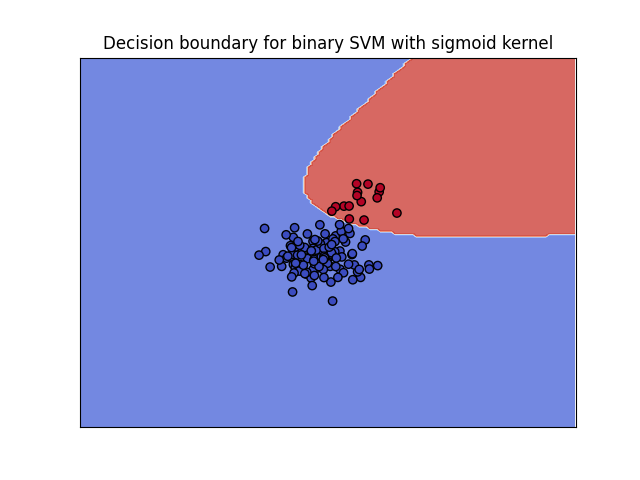
\includegraphics[width=\textwidth]{plots/sigmoid_binary.png}
        \caption{sigmoid Binary SVM}
    \end{subfigure}
    \caption{Binary SVM Decision Boundaries}
\end{figure}
\begin{figure}
    \centering
    \begin{subfigure}{0.45\textwidth}
        \centering
        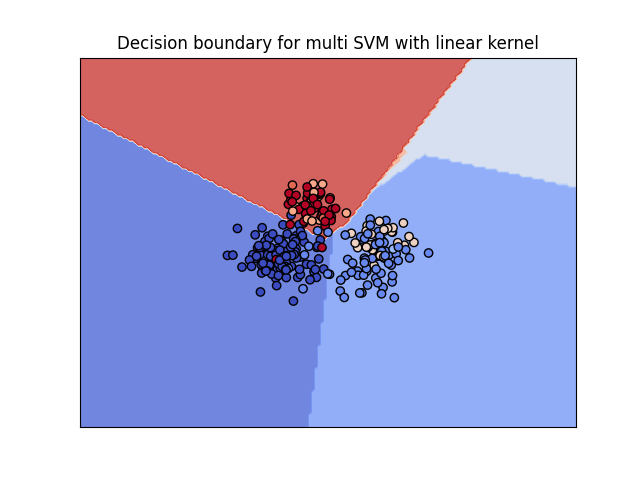
\includegraphics[width=\textwidth]{plots/linear_multi.png}
        \caption{Linear Multi-Class SVM}
    \end{subfigure}
    \begin{subfigure}{0.45\textwidth}
        \centering
        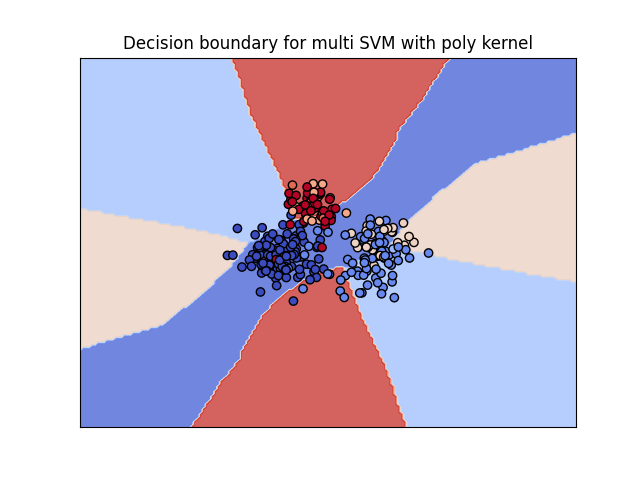
\includegraphics[width=\textwidth]{plots/poly_multi.png}
        \caption{Polynomial Multi-Class SVM}
    \end{subfigure}
    \begin{subfigure}{0.45\textwidth}
        \centering
        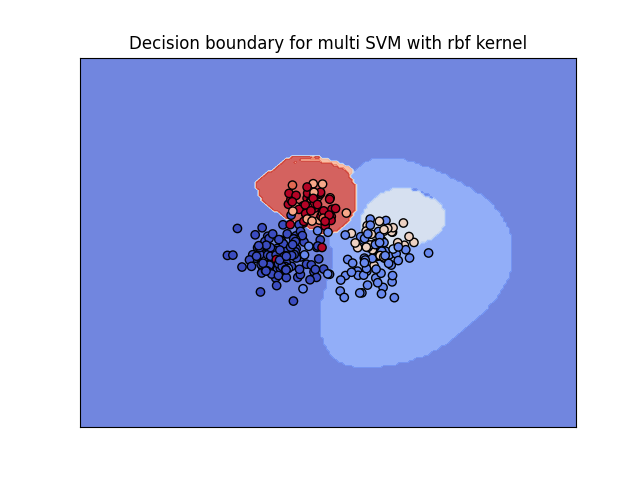
\includegraphics[width=\textwidth]{plots/rbf_multi.png}
        \caption{RBF Multi-Class SVM}
    \end{subfigure}
    \begin{subfigure}{0.45\textwidth}
        \centering
        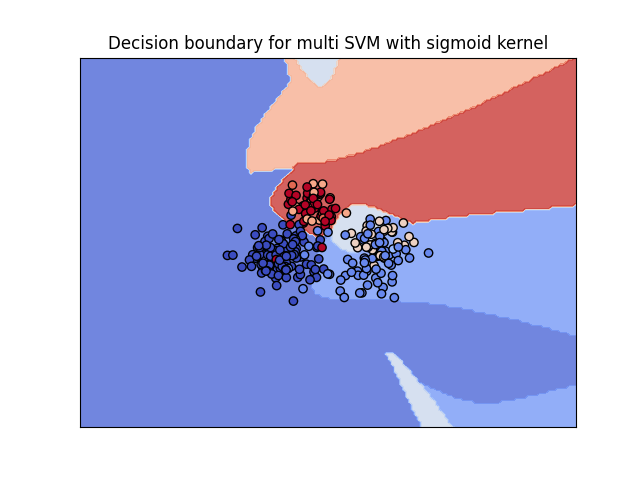
\includegraphics[width=\textwidth]{plots/sigmoid_multi.png}
        \caption{sigmoid Multi-Class SVM}
    \end{subfigure}
    \caption{Multi-Class SVM Decision Boundaries}
\end{figure}
\FloatBarrier 
\section{Conclusion}
This paper presented a methodology for creating Support Vector Machine (SVM) kernels from scratch using Python and NumPy.
We discussed the implementation of linear, sigmoid, polynomial, and radial basis function (RBF) kernels in a binary and multiclass SVM
and how Binary SVMs are used underneath the hood of multiclass SVMs. These kernels were tested on E. coli data and compared to the results
of the scikit-learn SVM implementation. The results show that the implemented kernels can often yield better accuracy than the scikit-learn
implementation; at the cost of increased training time. Kernel training times were ran multiple times and averaged to provide a more
accurate metric as training times were low and had a high variance. By harnessing the power of dimensionality reduction, we were
able to show the decision boundaries in 2 dimensions while still retaining the accuracy of higher dimensional data. These 
decision boundaries show how each kernel can affect the shape of the classification boundary and how the kernels can be used to
classify non-linear data.

\end{document}